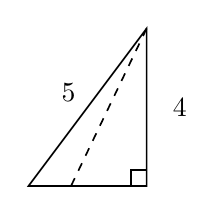
\begin{tikzpicture}[x=1cm,y=1cm,font=\normalsize,
 geometry edge/.style={solid,line width=.6pt},
 geometry mark/.style={solid,line width=.6pt},
 geometry label/.style={font=\normalsize,inner sep=2pt}]
\coordinate (L) at (-1.5,0);
\coordinate (R) at (0,0);
\coordinate (T) at (0,2);
\coordinate (Q) at (-0.96,0);
\draw[geometry edge] (L)--(R)--(T)--cycle;
\draw[geometry edge,dashed] (T)--(Q);
\draw[geometry mark] (-0.2,0)--(-0.2,0.2)--(0,0.2);
\node[font=\normalsize,inner sep=2pt,fill=white] at (-0.99,1.18) {$5$};
\node[font=\normalsize,inner sep=2pt,fill=white] at (0.42,1) {$4$};
\end{tikzpicture}
